\section{Applying WODA to the Open Legal Address File problem}
\label{crowdsourcing-olaf}

\subsection{How primary open data sources shape the solution}

The availability of high quality and authoritative open data is central to the definition of the solution. An assessment of available sources highlighted OS' "Open Names"\footnote{Ordnance Survey is the national mapping agency for Great Britain. See \url{https://www.ordnancesurvey.co.uk/business-and-government/products/os-open-names.html}.}, (OSON) as suitable primary input. 

OSON "lists definitive place names, roads numbers and postcodes in Great Britain", but not (i) which house names and numbers are in which road, and (ii) which house names and numbers are associated with which postcode. Therefore, OLAF can be seen as an augmentation of OSON, obtained by adding those missing components.

The production of the missing data can be achieved through running three complementary processes described in figure \ref{fig:problem_decomposition_2} as {\it p1}, {\it p2}\footnote{98\% of UK addresses are characterised by a house number rather than a house name, so tackling {\it p1} is substantially more relevant to OLAF's completeness than {\it p2}.} and {\it p3}. 

\begin{figure}
	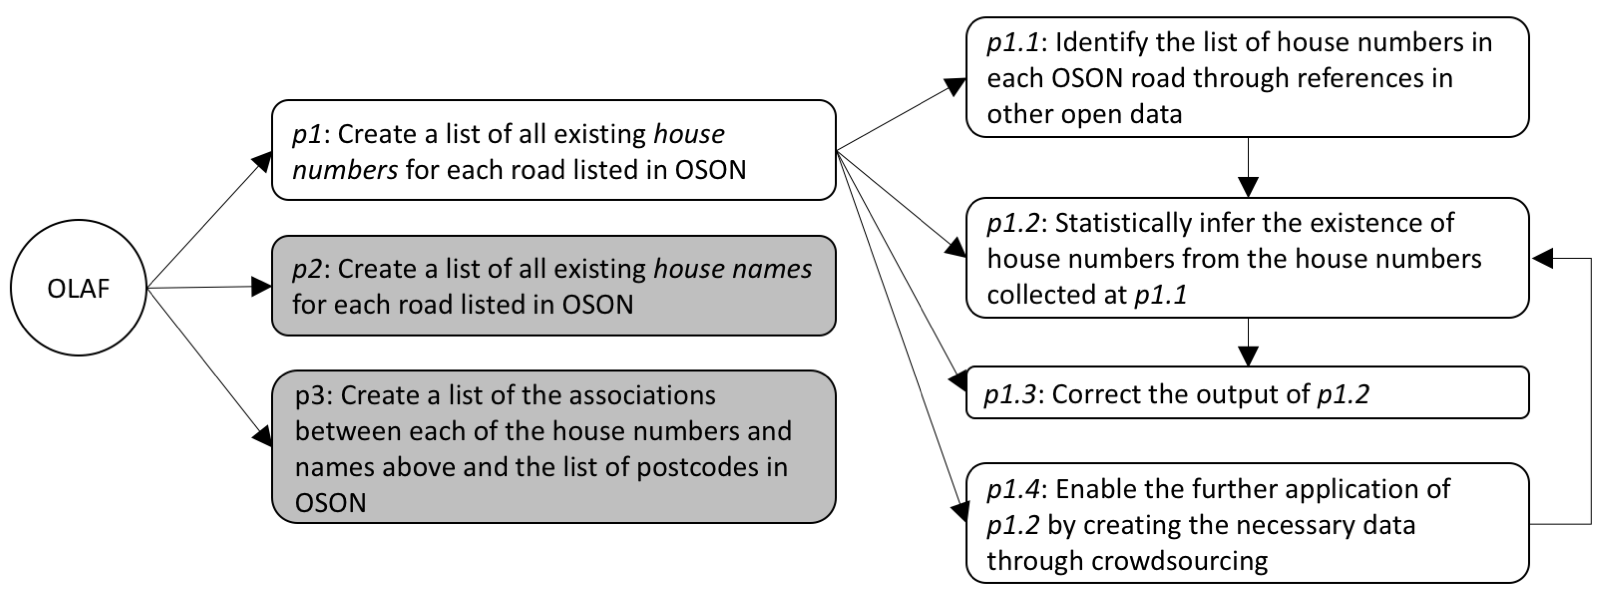
\includegraphics[width=1.0\textwidth]{problem-decomposition-2.png}
	\caption{A possible decomposition of OLAF}
	\label{fig:problem_decomposition_2}
\end{figure}

The partial availability of the missing data in other primary sources such as Land Registry's "Price Paid Data"\footnote{Land Registry is a non-ministerial UK Government department with the responsibility to register the ownership of land and property in England and Wales. See \url{https://www.gov.uk/government/collections/price-paid-data}.} enables to further refinement of process {\it p1} in four sub-processes {\it p1.1}, {\it p1.2}, {\it p1.3}\footnote{See \url{https://github.com/Digital-Contraptions-Imaginarium/OLAF-yr2_lab/blob/gh-pages/docs/README.md#error-in-inferred-house-numbers} for an assessment of the impact of error.} and {\it p1.4}. LRPP records every property ownership transfer in England and Wales since 1995, including their full addresses\footnote{LRPP is the largest open data source that include UK addresses.}, from which the inference of addresses is possible.

\subsection{The OLAF-specific workflow}

The generic workflow described in \ref{generic-workflow} can be specialised for OLAF by integrating {\it p1.1}, {\it p1.2} and {\it p1.4}. Figure \ref{fig:workflow_2} shows the new workflow and the mapping against the three processes. 

\begin{figure}
	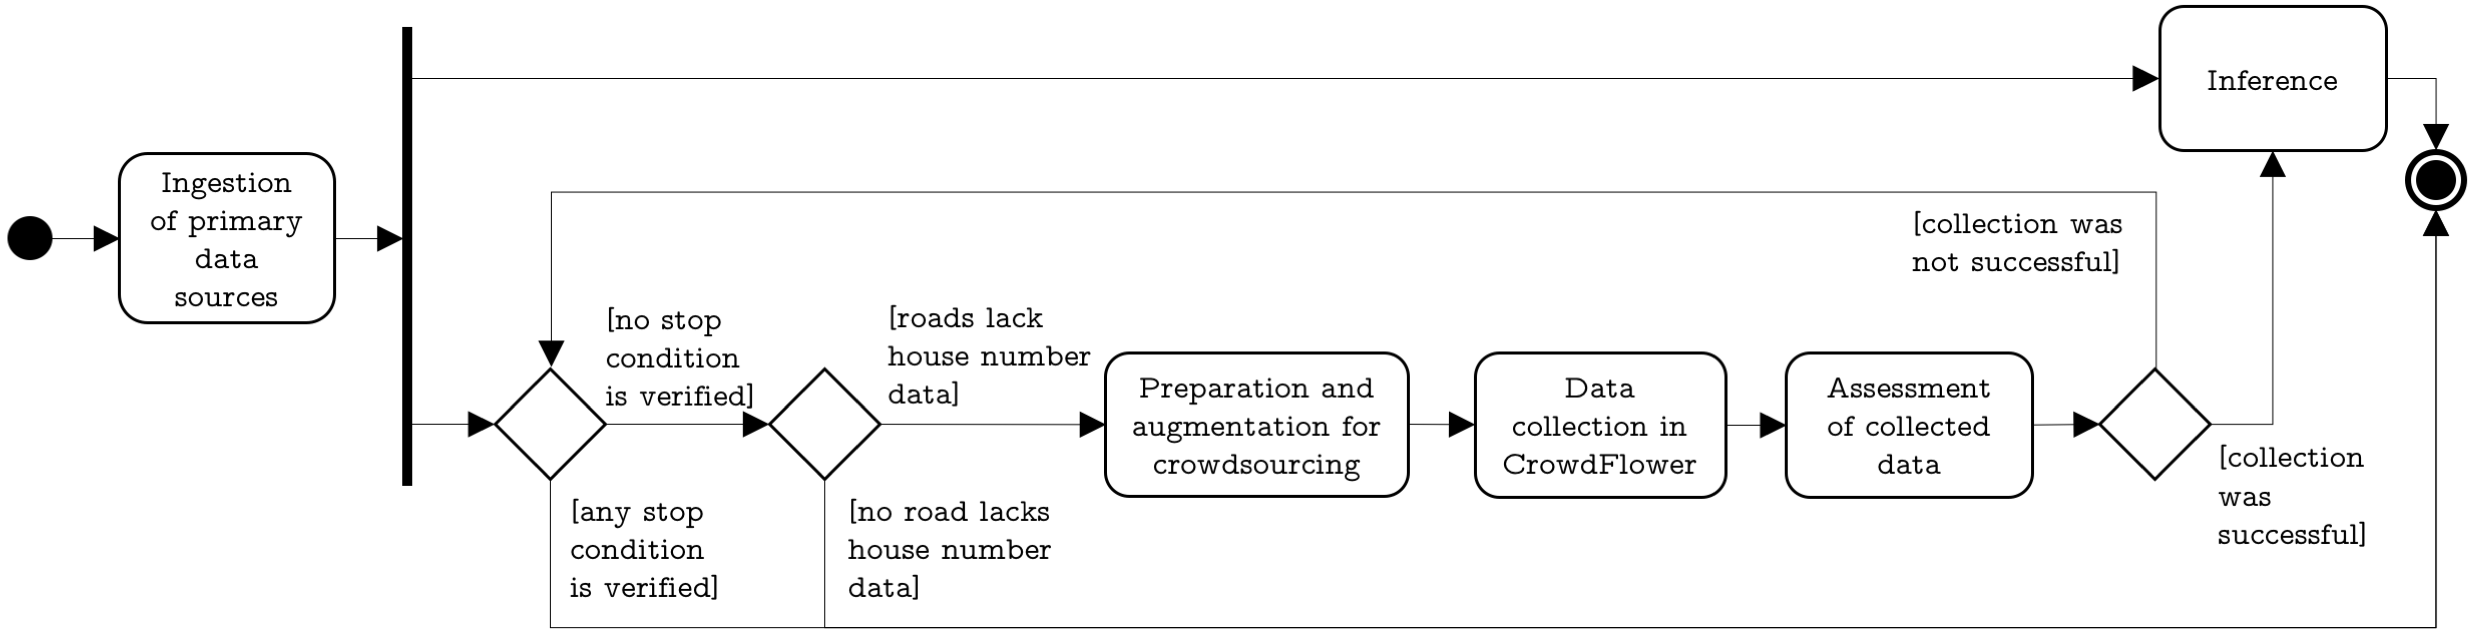
\includegraphics[width=1.0\textwidth]{workflow-2.png}
	\caption{UML process diagram of the OLAF-specific workflow to create house numbers}
	\label{fig:workflow_2}
\end{figure}

\subsection{Ingestion of primary data sources} 

Both OSON and LRPP contain references to streets, by their name. The main challenge of harvesting LRPP is to identify unambiguously the streets the house numbers are associated to, across the two datasets. Issues such as differences in spelling (e.g. "Downing Street" instead of "Downing St") and association of the locations not to the same town, but to localities thereof (e.g. "Clapham" instead of "London"), need being managed with common data processing practices.

\subsection{Inference} 
\label{inference-algorithms} 

\textbf{House numbering convention} Inferring house numbers is strictly dependent on the local numbering convention for the assignment of house numbers and names to buildings. In the UK, buildings are typically numbered sequentially starting from 1, at the extremity of the road closest to the town centre. Odd numbers are on the left-hand side, as seen from the town centre, while even number are on the right-hand side. House numbers can be suffixed by one or more letters: this is typical of larger buildings that at some point in time got divided into smaller dwellings. 
        
\textbf{Inference algorithms} Once the numbering convention is known, inference can be used to create a large volume of missing house numbers from the observation of known house numbers. Algorithms \ref{algo:inference-numbers} and \ref{algo:inference-numbers-suffix} below have a very high probability of correctly inferring the existence of house numbers\footnote{See \url{https://github.com/Digital-Contraptions-Imaginarium/OLAF-yr2_lab/blob/gh-pages/docs/README.md#exceptions-in-the-uk-house-numbering-system} for exceptions in the convention}. 

\vspace{5mm}

\begin{algorithm}[H]
    \KwData{The list of known house numbers in a road}
    \KwResult{The list of inferred house numbers in the same road}
    \eIf{the list includes at least one even and one odd number}{
        infer all numbers between the lowest and the highest known numbers\;
    }{
        \If{the list includes at least two even or two odd numbers}{
            infer all even/odd numbers between the lowest and the highest numbers\;
        }
    }
    \caption{Inference of house numbers}
    \label{algo:inference-numbers}
\end{algorithm}

\vspace{5mm}

\begin{algorithm}[H]
    \KwData{The list of known house numbers with suffixes in a road}
    \KwResult{The list of inferred house numbers with suffixes in the same road}
    \For{each house number appearing in the list with at least two suffixes}{
        infer all suffixes between the lowest and the highest known suffix, in alphabetical order\;    
    }
    \caption{Inference of house number with suffixes}
    \label{algo:inference-numbers-suffix}
\end{algorithm}

\subsection{Enabling inference for roads with no data} 

Inference of house numbers is enabled by one of the following two conditions: (a) the knowledge of two or more different house numbers in the same street and (b) the knowledge of two or more suffixes for the same number. The former has the highest potential to generate new house numbers.

When dealing with roads for which LRPP provides no data, it is useful to focus crowdsourcing on creating the conditions that enable that potential. To infer the largest sets of numbers it is necessary to use as input to algorithm \ref{algo:inference-numbers} the road's lowest and highest known house numbers\footnote{For simplicity, we did not consider (i) that it is also useful to know if the streets have both odd and even house numbers and (ii) the case where one house number only is known for a street, for which we could assume 1 to be the lowest house number.}.

\subsection{Stop conditions} 

The stop conditions referred to in the diagram are every condition not strictly related to the function of the system, e.g. the availability of budget. In other words, the workflow is iterated as long as budget is available, even if the aimed outcome is not achieved. 

\subsection{Preparation and augmentation for crowdsourcing} 

The data required by the crowdsourcing component may need preparation and augmentation before being used. In the case of OLAF, an additional primary data source is used to support the Workers in their tasks: OS' "Open Roads"\footnote{See \url{https://www.ordnancesurvey.co.uk/business-and-government/products/os-open-roads.html}.} (OSOR). 

OSOR is used to calculate the geographical coordinates of the extremities of the roads where the lowest and the highest house numbers are more likely to be found. These are offered as "points of interest" to support the crowdworkers in their search. It is an example of how open data can be used not necessarily as a direct input into producing the output dataset, but to support the human participants in their function, too.

\subsection{Data collection in CrowdFlower and assessment}

The crowdsourcing component of WODA can be configured to create the house numbers needed to enable inference. 

\textbf{Finding house numbers as a labelling exercise} Observing the imagery of a street to identify its lowest and highest house number is not conceptually different than crowdsourced annotation applications that extensively studied in literature, with the following exceptions:

\begin{itemize}
        
    \item For each item subject to annotation, two independent\footnote{One could argue that the two annotations are not truly independent, as the lowest house number is, by definition, lower than the highest house number. In practical terms, though, the task of surveying a street cannot leverage such mathematical relation. In other words, knowing what the highest house number is won't help the participant finding the lowest house number, as her finding is rather due to the observation of the topology of the street and the progression of nearby house numbers.} annotations rather than one are collected: the lowest and highest visible house numbers\footnote{It is not useful to as a participant to look for the lowest house number and another to look for the highest. By exploring the pictures, participants will naturally focus her research on the extremities of the road, where the relevant house numbers are, without knowing in advance which of the two she is finding first.}.
        
    \item The information subject to the annotation could be identified as existing, but the annotation may not be possible anyway\footnote{E.g. a participant may be able to identify the first house in a street, but vegetation may hide the number. There is also the possibility that the mapping provider coverage does not include the surveyed street. Moreover, unlike other countries, in the UK local authorities do not provide house number plates to the building owners, so this remains their responsibility. Building owners have the option not to affix any plate at all.}.
        
    \item The road to survey may be no buildings\footnote{Because of how the workflow was defined, crowdsourcing is used on streets of which there is little or no reference in LRPP over the last 20 years. This means that the road is likely rural and have few buildings.}.
        
\end{itemize}

The following is a description of the approach that was used for crowdsourcing addresses, that is common to all experimental conditions that were tested.

\subsubsection{Task model} \leavevmode \\ %% Why is this necessary to get a new line?

\textbf{Requester.} The Requester desires to gather the lowest and the highest house numbers that can be observed in a specified street, as they can be intelligibly identified by browsing pictures of the street. Alternatively, if no two house numbers are identifiable, the Requester needs being informed, too. Different streets have different degree of interest to the Requester, who is interested in prioritising the collection of the data for the higher interest streets in respect to the lower interest ones. The Requester requires the help of human agents to carry out the tasks, that we will call Workers in the following.

\textbf{Task.} Each HIT (Human Intelligence Task) consists of browsing the pictures of a street until achieving reasonable certainty of having identified the lowest and the highest house numbers or, alternatively, the lack thereof.

\textbf{Strategy.} 
The strategy relies on traditional crowdsourcing techniques for image labelling.

\textbf{Crowd $\rightarrow$ Worker.} Each Worker provides judgement on a task by browsing the pictures and declaring if she has found the lowest and the highest house numbers or none. Multiple Workers are asked to identify the house numbers for the same street. The resulting data is chosen through majority voting.

\textbf{Quality.} Quality is defined by a combination of (a) accuracy of the Workers in responding to tests questions, and (b) consensus in the data submitted through repeated surveys of the same road. Aggregation takes place accordingly as explained below.

\subsubsection{Workers quality}
    
Probing Workers using conventional test questions - e.g. where the correspondence of the Worker submissions is checked vs the same data collected by the research team as described in \cite{Kittur:2008gj} - would be a powerful tool to identify high vs low quality contributors, but is very expensive in OLAF's case. The task of surveying a street is not trivial, and early anecdotal evidence from early tests of the implementation showed many Workers leaving after performing no more than two or three surveys. To further damage the performance of the system, the ones who stayed longer started cheating, or showed a substantial drop in their performance. This suggested that spending a substantial part of the Worker's effort on test questions - e.g. making one out of three surveys a test - was not affordable.

Not using any kind of test question is unlikely to be successful, too, and it was explored in previous work such as \cite{DellaPenna:tf}. As an alternative, though, simple test questions can be set up on data that is already available, in a way that is similar to classic anti-spamming techniques like CAPTCHAs as described in \cite{Difallah:2012ty}. In OLAF's case the name of the street itself is used: Workers are asked to copy and paste or type the name of the street as part of their survey. Workers that do not achieve the target accuracy are excluded from further work.

\subsubsection{Results aggregation}

Repeated surveys of the same road are equivalent to the use of repeated judgement in conventional image labelling exercises. This practice is described extensively in literature and demonstrate that the results produced by a few expensive expert individuals are comparable to what emerges from involving multiple answers by crowds of non-expert Workers, e.g. in \cite{Snow:2008wo} and \cite{Sheng:2008gra}. As the answers are inevitably noisy, different Workers were asked to survey the same road, and their responses are aggregated to decide what is the most likely and truthful observation. 
        
Approaches to aggregation are an equally well studied subject, and a majority decision is a natural option (e.g. \cite{Le:2010ug}). The detailed parameters and process of how consensus is defined and calculated are tuned for better performance and address issues specific to the context (e.g. in \cite{Hirth:2011fh}). 

In the case of OLAF, consensus is measured by using Fleiss' kappa statistics for inter-annotator agreement, as described for example in \cite{Nowak:2010gt}. For those streets where the house numbers {\it were} found, a kappa of 60\% on at least 5 surveys is sufficient consensus (e.g. see \cite{Landis:1977kv}). For those streets where the house numbers were {\it not} found, a kappa of 80\% on at least 10 surveys is required instead, as it is more likely that unreliable Workers agree in reporting that.

The number of 5 and 10 judgements is chosen because they are respectively the minimum number of judgements where 60\% and 80\% kappa can be achieved without the need of an unanimous agreement (4 vs 1 for 60\% and 9 vs 1 for 80\%). 

Rounds of 5 surveys per road are performed until consensus is reached on both its lowest and highest house numbers. Because of the nature of the task, new surveys are performed even if consensus is reached already on either of the two numbers.  

\subsubsection{Recruitment}

We sourced all our Workers from CrowdFlower. For each experiment, we created one dedicated CrowdFlower job. We used identical settings for each experiment set, consisting of the following parameters:

\textbf{Geography} Limited to the top 10 contributor countries in CrowdFlower where English is an official or officially recognised language\footnote{See \url{https://success.crowdflower.com/hc/en-us/articles/202703345-Crowd-Demographics}, the identification of the countries was last repeated on 19 December 2015, before the running the experiments described in this paper. The list of countries is: Bangladesh, Canada, India, Malaysia, Netherlands, Pakistan, Philippines, Sri Lanka, United Kingdom and United States of America.}.

\textbf{Skills} We chose Workers from the default CrowdFlower performance category (formerly named "level 2"), that accounts for 29\% of the total population\footnote{See \url{https://success.crowdflower.com/hc/en-us/articles/202703345-Crowd-Demographics}, the calculation was done on 19 December 2015.}.

\textbf{Accuracy} As described in the previous section, as a test question Workers were asked to copy and paste or type the name of the street as part of their submission in each task. Being the question this simple, error was not accepted the requested accuracy was 99\%\footnote{CrowdFlower does not allow the Requester to set target accuracy to 100\%.}.

\textbf{Judgements} In groups of 5 per road, repeated until consensus is reached, by different Workers without repetition. Each Worker is allowed to contribute to as many tasks as possible.

\textbf{Behaviour} Each Worker was paid for 1 task, and 1 task is made of 1 street to survey.

\textbf{Reward / Time Limits} The reward was 0.20 US Dollars per task. Workers requiring less than 90 seconds per task were considered at high risk of being malicious and excluded to perform additional tasks. CrowdFlower imposes a time limit of 30 minutes maximum per task.

\subsection{Implementation}

\begin{sloppypar} %% see http://tex.stackexchange.com/questions/54946/how-to-break-long-url-in-an-item#comment114992_54949
The code implementing WODA and detailed documentation can be found in the following GitHub repositories: (i) ingestion and preparation of the reference data at \url{https://github.com/Digital-Contraptions-Imaginarium/OLAF-yr2_reference_data}, (ii) inference of house numbers at \url{https://github.com/Digital-Contraptions-Imaginarium/OLAF-yr2_inference_data}, (iii) instructions video for the Workers at \url{https://github.com/Digital-Contraptions-Imaginarium/OLAF-yr2_lab_instructions-video} and (iv) preparation of the data for crowdsourcing and elaboration of the results at \url{https://github.com/Digital-Contraptions-Imaginarium/OLAF-yr2_lab}, in the {\it data-prep-scripts} and {\it analysis-scripts} folders respectively. All code is released under the MIT licence, and any other asset under CC BY 4.0 International.
\end{sloppypar}